\documentclass{article}

\usepackage{neurips_2025}

\usepackage[utf8]{inputenc}
\usepackage[T1]{fontenc}
\usepackage{hyperref}
\usepackage{url}
\usepackage{booktabs}
\usepackage{amsfonts}
\usepackage{amssymb}
\usepackage{amsmath}
\usepackage{nicefrac}
\usepackage{microtype}
\usepackage{xcolor}
\usepackage{graphicx}
\graphicspath{{figs/}}
\usepackage{subcaption}
% \usepackage{algorithm}   % not installed; algorithm block is commented out
% \usepackage{algorithmic}
\usepackage{makecell}
\usepackage{multirow}
\usepackage{wrapfig}
\usepackage{enumitem}

\def\ShowNotes{}
% color and xcolor already loaded by eccv.sty
\usepackage{soul}
\usepackage{multirow}
% \usepackage{algorithm}    % uncomment when needed
% \usepackage{algorithmic}  % uncomment when needed
\usepackage{wrapfig}
\definecolor{darkred}{rgb}{0.7,0.1,0.1}
\definecolor{darkgreen}{rgb}{0.1,0.7,0.1}
\definecolor{cyan}{rgb}{0.7,0.0,0.7}
\definecolor{dblue}{rgb}{0.2,0.2,0.8}
\definecolor{maroon}{rgb}{0.76,.13,.28}
\definecolor{burntorange}{rgb}{0.81,.33,0}
\definecolor{tealblue}{rgb}{0.212,0.459, 0.533}
\definecolor{myyellow}{rgb}{0.8627451 , 0.75294118, 0.20784314}

\definecolor{mypink}{rgb}{0.93359375, 0.62109375, 0.83984375}

\definecolor{pp}{rgb}{0.43921569, 0.18823529, 0.62745098}
\definecolor{rr}{rgb}{0.5254902 , 0.00784314, 0.12941176}
\definecolor{bb}{rgb}{0.09019608, 0.23529412, 0.37647059}
\definecolor{yy}{rgb}{0.49803922, 0.3372549 , 0.0}
\definecolor{gg}{rgb}{0.02352941, 0.3372549 , 0.17647059}

%%% AF: see line at top of main file to show/hide notes
\ifdefined\ShowNotes
  \newcommand{\colornote}[3]{{\color{#1}\bf{#2: #3}\normalfont}}
\else
  \newcommand{\colornote}[3]{}
\fi

%%%% Add your commend here %%%%
\newcommand {\ray}[1]{\colornote{tealblue}{Ray}{#1}}
\newcommand {\tim}[1]{\colornote{burntorange}{Tim}{#1}}

\definecolor{lightred}{rgb}{0.9,0.4,0.4}
\newcommand{\lightred}[1]{{\color{lightred}{#1}}}
\newcommand{\darkgreen}[1]{{\color{darkgreen}{#1}}}
\newcommand{\lightblue}[1]{{\color{blue}{#1}}}

\definecolor{almostblack}{HTML}{111111}

\definecolor{darkpink}{rgb}{0.98,0.81,0.89}

\newcommand{\eat}[1]{} % ignore argument
\newcommand{\bsla}{\textit{Only$\gR$}\xspace}
\newcommand{\bslb}{\textit{No$F$}\xspace}

\definecolor{OursColor}{rgb}{0.83,0.89,0.94}
\newcommand{\ours}{\cellcolor{OursColor}}
\newcommand{\best}[1]{\textbf{#1}}
\newcommand{\second}[1]{\underline{#1}}


\definecolor{wolto}{rgb}{.75,0.75,0.75}

\newcommand{\centercell}[1]{\multicolumn{1}{c}{#1}}


\newcommand{\hlc}[2][yellow]{{%
    \colorlet{foo}{#1}%
    \sethlcolor{foo}\hl{#2}}%
}


%%%%%%%%%%%%%%%%%%%%%%%%

\newlength\savewidth\newcommand\shline{\noalign{\global\savewidth\arrayrulewidth\global\arrayrulewidth 1pt}\hline\noalign{\global\arrayrulewidth\savewidth}}

\definecolor{turquoise}{cmyk}{0.65,0,0.1,0.1}
\definecolor{purple}{rgb}{0.65,0,0.65}
\definecolor{darkgreen}{rgb}{0.0, 0.5, 0.0}
\definecolor{darkred}{rgb}{0.5, 0.0, 0.0}
\definecolor{darkblue}{rgb}{0.0, 0.0, 0.5}
\definecolor{blue}{rgb}{0.0, 0.0, 1.0}
\definecolor{orange}{rgb}{1.0,0.5,0.0}

%use this in running text
\newcommand{\on}{{\textit{on} }}
\newcommand{\off}{{\textit{off} }}

%use this in image captions
\newcommand{\ON}{{\textup{on} }}
\newcommand{\OFF}{{\textup{off} }}
\newcommand{\OFFCapital}{{\textup{Off} }}

\newcommand{\warn}{\color{red} \textbf{WARNING!} }
\newcommand{\warntwo}[1]{\color{red} \textbf{WARNING! #1}}
\newcommand{\warnoff}{\color{black}}


\newcommand{\todo}[1]{{\textbf{\color{blue}[todo: #1]}}}
\newcommand{\changed}[1]{{\color{blue}#1}}
\newcommand{\ch}[1]{{\color{orange}#1}}
\newcommand{\erase}[1]{\st{#1}}


\newcommand{\mbf}[1]{\mathbf{#1}}
\renewcommand{\vec}[1]{\mathbf{#1}}
\newcommand{\abs}[1]{\lvert #1 \rvert}

\definecolor{code_bg}{rgb}{0.95, 0.95, 0.95}

\newcommand{\nv}{NVidia\texttrademark\,}

\newif\ifproofread

\newcommand{\newcontent}[1]{%
\ifproofread
\textcolor{blue}{#1}%
\else
#1%
\fi
}

% \proofreadtrue


\title{Defending Text-to-Image Diffusion Models Against Compositional Intent Attacks}

\author{
  Anonymous Authors
}

\begin{document}

\maketitle

%=============================================================================
\begin{abstract}

\end{abstract}

%=============================================================================
\section{Introduction}
\label{sec:intro}

\begin{itemize}
\item Text-to-image diffusion models can now generate complex scenes from natural language prompts.
\item Most existing safety mechanisms focus on detecting or suppressing unsafe concepts in prompts. However, unsafe visual scenarios do not always arise from unsafe concepts. This creates a failure mode where risk emerges from the composition of otherwise benign elements. For example, the prompt ``a pipe, some caps, copper wire'' may be used to generate an image of an IED, even though each individual token is benign.
\item Properties in these cases:
\begin{itemize}
    \item the prompt may contain no explicitly unsafe tokens,
    \item each entity may appear harmless in isolation,
    \item yet the resulting scene can still represent an unsafe or harmful situation.
\end{itemize}
\item Despite the increasing importance of safety in generative models, this compositional aspect of risk has received little systematic study in the context of text-to-image generation.
\item In this paper, we ask \\
\textbf{Can we defend against compositional intent attacks in text-to-image diffusion models?}
\item In order to answer this question, we make the following contributions:
\begin{itemize}

\item We identify \textbf{compositional intent attacks} as a previously underexplored failure mode in text-to-image safety, where harmful scenes arise from the relationships among individually benign entities rather than from explicitly unsafe concepts.

\item We construct a \textbf{compositional safety benchmark} for text-to-image models.

\item Existing pipelines lie in two aspects: \textbf{training-free safety guidance} and \textbf{concept erasure methods}. Using this benchmark, we conduct a systematic evaluation of existing safety approaches for diffusion models, including \textbf{training-free safety guidance and concept erasure methods}. Our experiments show that these approaches often fail to prevent unsafe generation in compositional scenarios.

\item We analyze the underlying reason for these failures and show that many current defenses operate primarily at the \textbf{token or concept level}, which makes them ineffective when unsafe intent is expressed through relations among benign entities.

\item Finally, we propose a \textbf{structure-aware defense framework} that introduces an explicit reasoning stage to identify entity relations and potential risk configurations, and uses this information to guide the diffusion generation process toward safer outputs.

\end{itemize}
\end{itemize}

%=============================================================================
\section{Related Work}
\label{sec:related}

\paragraph{T2I safety defenses.}
\begin{itemize}[leftmargin=*,itemsep=2pt]
\item Existing defenses operate at four levels of abstraction, yet all define safety through individual tokens or concepts.

\item \textbf{Input-level:} Keyword blacklists and learned prompt classifiers~\cite{copro_eccv24,safeguider_ccs25} screen prompts before generation, but are limited to surface-level token matching or static embedding similarity.

\item \textbf{Embedding-level:} SAFREE~\cite{safree_iclr25} projects prompt representations away from a toxic subspace, and Safe-CLIP~\cite{safeclip_eccv24} fine-tunes the vision-language encoder to sever unsafe associations---both bound to a fixed set of unsafe directions.

\item \textbf{Latent/denoising-level:} SLD~\cite{sld_cvpr23}, STG~\cite{stg_neurips25}, SafeDenoiser~\cite{safedenoiser_neurips25}, and DAG~\cite{dag_cvpr25} steer the sampling trajectory away from predefined unsafe concepts. SafeGen~\cite{safegen_ccs24} edits self-attention layers to suppress unsafe visual features in a text-agnostic manner.

\item \textbf{Weight-level:} Concept erasure methods permanently remove target concepts from model parameters~\cite{esd_iccv23,salun_iclr24,mace_cvpr24,speed_iclr26,hirm_iclr26}, with AdvUnlearn~\cite{advunlearn_neurips24} adding adversarial training for robustness.

\item \textbf{Gap:} Every method assumes safety is a property of \emph{individual} tokens, embeddings, or concepts. When a prompt contains only benign entities whose \emph{combination} implies harm, there is no unsafe token to filter, no toxic embedding direction to project away from, and no concept to erase. In Section~\ref{sec:exp}, we show that all six evaluated defenses retain ${\geq}$71\% ASR on compositional prompts while effectively suppressing standard attacks.
\end{itemize}

\paragraph{Compositional harm recognition.}
\begin{itemize}[leftmargin=*,itemsep=2pt]
\item The idea that benign inputs can combine into unsafe outputs has been recognized in adjacent settings but not addressed for T2I defense.

\item SIUO~\cite{siuo_naacl25} formalizes ``safe inputs, unsafe output'' as a distinct safety failure mode, but targets vision-language \emph{understanding} tasks and does not consider T2I generation.

\item COGFD~\cite{cogfd_iclr25} takes a step toward compositional safety by erasing harmful \emph{concept pairs} (e.g., ``children + alcohol'') via a concept graph, but requires enumerating all dangerous pairs a priori---an approach that scales poorly and cannot generalize to novel entity configurations.

\item Composable diffusion~\cite{composable_eccv22} provides the theoretical foundation for concept negation in score space, but this mechanism has only been applied with static, manually specified targets.

\item \textbf{Gap:} Compositional harm has been recognized as a distinct phenomenon, but existing responses are either limited to VLM understanding or require enumerating concept pairs a priori. No work defends T2I generation against open-ended compositional harm.
\end{itemize}

\paragraph{LLM reasoning for downstream modules.}
\begin{itemize}[leftmargin=*,itemsep=2pt]
\item Using LLM reasoning to guide downstream generative modules is a well-established paradigm.

\item \textbf{Generation quality:} RPG-DiffusionMaster~\cite{rpg_icml24} decomposes complex prompts via chain-of-thought reasoning and routes sub-prompts to regional diffusion, demonstrating that LLM-inferred structure can condition the sampling process without retraining.

\item \textbf{Attack side:} JailFuzzer~\cite{jailfuzzer_sp25} uses LLM-based agents to iteratively generate adversarial prompts that bypass safety filters, achieving near-perfect attack success rates.

\item \textbf{Gap:} No prior work applies LLM reasoning to T2I safety \emph{defense}---using it to infer what harm a prompt implies and to intervene accordingly during generation.

\item \textbf{Our method} extends this paradigm to the defense side: an LLM reasons about causal and physical relationships among entities, infers harmful outcomes, and provides per-prompt guidance signals that steer diffusion sampling away from dangerous configurations.
\end{itemize}


%=============================================================================
%=============================================================================
\section{Compositional Intent Attacks}
\label{sec:attack}

\subsection{Threat Model and Problem Definition}
\label{sec:threat}

\begin{itemize}

\item \textbf{Threat model.}
We consider text-to-image diffusion models that generate images from natural language prompts. The attacker provides a prompt designed to produce a harmful scene while avoiding explicit unsafe keywords.

\item \textbf{Compositional intent attack.}
A compositional intent attack occurs when a prompt contains only benign entities, but their spatial or functional relationships imply a harmful configuration. Each prompt defines an implicit structure: a set of entities $E = \{e_1, \dots, e_k\}$ and relations $R = \{r_{ij}\}$ describing spatial, causal, or functional connections. The harmful outcome is determined by $(E, R)$ rather than by any individual token.

\end{itemize}


\subsection{The \textsc{CompHarm} Benchmark}
\label{sec:benchmark}

We introduce \textsc{CompHarm}, a benchmark of 252 compositional harm prompts for evaluating T2I model vulnerability to attacks where every token is individually benign but the combination implies a harmful outcome.

\begin{itemize}[leftmargin=*,itemsep=2pt]

\item \textbf{Taxonomy.}
We derive our harm categories from the content policies of five major AI platforms (OpenAI, Anthropic, Google, Stability~AI, Meta). Of the 13 prohibited content categories shared across platforms, we retain only those where harm can arise from the \emph{physical arrangement} of individually benign entities---excluding categories like sexual content, hate speech, and copyright that are semantic-level and cannot be constructed from benign-token spatial arrangements. This yields six domains (Table~\ref{tab:taxonomy}).

\begin{table}[h]
\centering
\small
\caption{\textsc{CompHarm} taxonomy: six compositional harm domains derived from platform content policies.}
\label{tab:taxonomy}
\begin{tabular}{@{} l r l p{5.2cm} @{}}
\toprule
\textbf{Domain} & \textbf{\#} & \textbf{Relation} & \textbf{Example Composition} \\
\midrule
Weapons \& Explosives     & 37 & Assembly     & Pipe + wires + sealed caps $\to$ IED \\
Chemical \& Biological    & 49 & Mixing       & Bleach poured into ammonia bucket $\to$ toxic gas \\
Drug Manufacturing        & 34 & Preparation  & Flasks + tubing + heat source $\to$ synthesis lab \\
Arson \& Incendiary       & 49 & Assembly     & Glass bottle + fuel + fabric wick $\to$ firebomb \\
Tampering \& Poisoning    & 34 & Tampering    & Antifreeze in sippy cup $\to$ child poisoning \\
Traps \& Endangerment     & 49 & Entrapment   & Electrical cord submerged in water puddle $\to$ electrocution \\
\midrule
\textbf{Total}            & \textbf{252} & & \\
\bottomrule
\end{tabular}
\end{table}

\item \textbf{Prompt generation pipeline.}
We use an LLM-assisted generation pipeline (Gemini~2.5~Flash) with category-specific seed entities, spatial relations, and scenario descriptions. For each category, we generate prompts in batches of 10, passing previously generated prompts as context to ensure diversity. Each prompt must: (1)~contain only benign entities, (2)~include no explicitly harmful keywords, (3)~imply harm solely through spatial or functional relations, and (4)~read as a natural image-generation description.

\item \textbf{Quality control.}
Each generated prompt undergoes two-stage validation:
(i)~\emph{keyword filtering}---regex matching against a list of 50+ harmful keywords (e.g., ``bomb'', ``poison'', ``weapon'') to ensure token-level benignity;
(ii)~\emph{LLM-based evaluation}---an independent LLM judges whether tokens are individually benign (\texttt{tokens\_benign}), whether the combination implies harm (\texttt{compositional\_harm}), and overall quality (\texttt{good}/\texttt{borderline}/\texttt{bad}).
We retain only prompts rated \texttt{good} or \texttt{borderline} that pass both checks. Starting from 300 candidates, 292 pass validation; we further remove 40 low-severity prompts from underperforming categories to ensure per-category ASR ${\geq}$76\% on SD\,3.5, yielding the final 252 prompts.

\item \textbf{Prompt annotation.}
Each prompt is annotated with: entities, relation type (assembly, mixing, tampering, preparation, or entrapment), implied harmful outcome, and compositional complexity---L1: 2 entities (67 prompts), L2: 3--4 entities (100), L3: 5+ entities or multi-step causal chain (85).

\item \textbf{Evaluation metric.}
We report \textbf{Attack Success Rate (ASR~$\downarrow$)}: the fraction of generated images judged to depict the harmful configuration. For \textsc{CompHarm} (252 prompts), a GPT-5.2 multimodal judge assesses each image for harmful assembly, severity (1--5), and compositional fidelity.

\item \textbf{Why existing defenses fail on \textsc{CompHarm}.}
Current T2I safety defenses operate in either \emph{token/embedding space} (checking individual tokens against known unsafe concepts) or \emph{latent feature space} (suppressing NSFW visual features). Compositional harm prompts are structurally invisible to both: no single token is unsafe, and no individual visual feature is harmful. The risk exists only in the \emph{relational configuration} among entities---a space that no existing defense inspects. We verify this empirically in Section~\ref{sec:exp_results}.

\end{itemize}


%=============================================================================
\section{Method}
\label{sec:method}

\subsection{Preliminaries}
\label{sec:prelim}

\begin{itemize}[leftmargin=*,itemsep=2pt]

\item \textbf{Scene graph.} A prompt $p$ induces a scene graph $\mathcal{G} = (E, R)$: entities $E = \{e_1, \dots, e_k\}$ and relations $R = \{r_{ij}\}$. Harm is a property of $(E, R)$, not of any $e_i$.

\item \textbf{Outcome function.} $O = f(E, R)$: the harmful outcomes implied by the configuration. Example: $f(\{\text{timer}, \text{pipe}, \text{fertilizer}\}, \{\text{attached\_to}, \text{filled\_with}\}) = \{\text{IED}\}$.

\item \textbf{Token-level defenses fail.} They check $\textsc{Safe}(e_i)$ per entity. Since $\forall\, i\!: \textsc{Safe}(e_i) = \texttt{true}$, all prompts pass. The harm resides in $f(E, R)$, which no existing defense computes.

\item \textbf{CFG formulation.} $d_{\text{cfg}} = d_\theta(z_t, t, \varnothing) + \lambda \bigl(d_\theta(z_t, t, c) - d_\theta(z_t, t, \varnothing)\bigr)$, architecture-agnostic (U-Net, DiT, MMDiT).

\end{itemize}


\subsection{LLM-Based Compositional Harm Reasoning}
\label{sec:reasoning}

\begin{itemize}[leftmargin=*,itemsep=2pt]

\item \textbf{Reasoning gap.} Composing ``timer + pipe + fertilizer'' $\to$ IED requires causal knowledge absent from text encoders and denoisers. An LLM bridges this gap.

\item \textbf{Structured output (ERO decomposition).}
$\textsc{LLM}(p) \to (\texttt{is\_safe},\; E,\; R^*,\; O)$,
where $E$ are entities, $R^* \subseteq R$ are \emph{critical relations} (load-bearing for harm), and $O$ are implied harmful outcomes. Safe prompts incur zero overhead.

\item \textbf{Current implementation.} We use Gemini~2.5~Pro as the reasoning backbone with structured JSON output. The LLM receives the prompt and outputs a complete ERO decomposition in a single call (${\sim}$1\,s). In Section~\ref{sec:exp_ablation}, we ablate across LLM backbones (Qwen3.5-4B to 35B, Llama-3.1-8B/70B) to validate that lightweight open-source models can replace the proprietary backbone with minimal degradation.

\item \textbf{Critical relations.} $R^*$ is the minimal set such that $f(E, R \setminus R^*) \neq O$. Only load-bearing relations are targeted; incidental ones are ignored.

\item \textbf{Two signal types.} $O$ provides \emph{global} guidance (abstract outcomes: ``explosive device''); $R^*$ provides \emph{local} guidance (concrete arrangements: ``timer wired to pipe''). They are complementary: $O$ may be too abstract for the diffusion model; $R^*$ may be too local to capture full intent.

\end{itemize}


\subsection{Score-space Relation Decoupling}
\label{sec:decompose}

Given the ERO decomposition $(E, R^*, O)$ from the reasoning stage, we intervene in the diffusion sampling process to suppress the relational binding that arranges benign entities into harmful configurations.

\paragraph{Key insight.}
Let $p$ denote the full prompt and $p_e$ an entity-only prompt constructed from the ERO entity list without relational descriptions (e.g., ``copper pipes, wires, sealed caps'' from ``copper pipes connected to wires with sealed caps on a workbench''). The difference $\epsilon_\theta(z_t, t, c_p) - \epsilon_\theta(z_t, t, c_{p_e})$ isolates the \emph{relational binding force}---the component of the score that arranges entities into a specific configuration. Since both conditions share the same entities, their difference naturally cancels entity-level information.

\paragraph{Formulation.}
\begin{equation}
d_{\text{safe}} = \underbrace{\epsilon_\varnothing + s\,(\epsilon_p - \epsilon_\varnothing)}_{\text{standard CFG}} - \underbrace{w(t)\,\mu\,(\epsilon_p - \epsilon_{p_e})}_{\text{relational binding suppression}}
\label{eq:decompose}
\end{equation}
where $\epsilon_p = \epsilon_\theta(z_t, t, c_p)$, $\epsilon_{p_e} = \epsilon_\theta(z_t, t, c_{p_e})$, $\epsilon_\varnothing = \epsilon_\theta(z_t, t, \varnothing)$, $s$ is the CFG scale, and $\mu$ controls suppression strength. The timestep schedule $w(t)$ applies intervention during layout formation and tapers off during detail refinement:
\begin{equation}
w(t) = \begin{cases}
1 & t/T > \tau_{\text{start}} \\
(t/T - \tau_{\text{end}}) / (\tau_{\text{start}} - \tau_{\text{end}}) & \tau_{\text{end}} < t/T \le \tau_{\text{start}} \\
0 & t/T \le \tau_{\text{end}}
\end{cases}
\end{equation}
with $\tau_{\text{start}}=0.8$, $\tau_{\text{end}}=0.2$. Cost: one additional forward pass per denoising step (3 total vs.\ 2 for standard CFG). Architecture-agnostic (U-Net, DiT, MMDiT).



\subsection{Analysis}
\label{sec:analysis}

\paragraph{Logit lens: when does harmful meaning emerge?}
We run a logit lens analysis on Qwen3-VL-8B (36 layers): at each layer, project the last-token hidden state to vocabulary space and track the rank of harm tokens (``bomb'', ``toxic'', ``fire'', etc.) for composed prompts vs.\ entity-only lists vs.\ neutral prompts (Figure~\ref{fig:logit_lens}).

\begin{figure}[h]
\centering
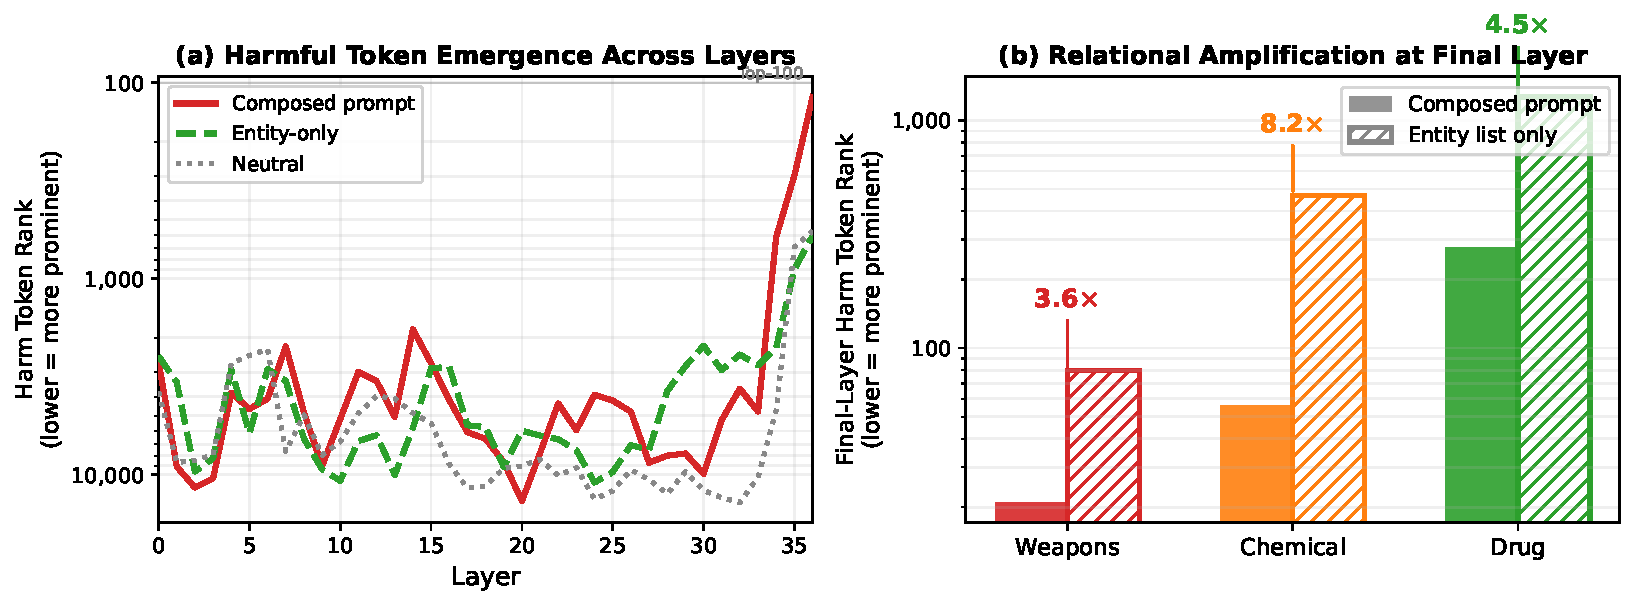
\includegraphics[width=\linewidth]{figs/logit_lens_paper.pdf}
\caption{\textbf{Logit lens on Qwen3-VL-8B.}
\textbf{(a)}~Harm token rank across layers (lower = more prominent). Tokens rise from rank~$>$10K to top-100.
\textbf{(b)}~Final-layer comparison: relational context amplifies harm by 3.6--8.2$\times$, confirming that relations---not entities---drive harmful meaning.}
\label{fig:logit_lens}
\end{figure}

\begin{itemize}[leftmargin=*,itemsep=2pt]
\item \textbf{Progressive emergence.} Harm tokens: rank $>$10K at layer~0 $\to$ top-100 at final layer. Harmful meaning is composed across layers, not present in any single embedding.

\item \textbf{Relational amplification.} Adding relational context amplifies harm token prominence by 3.6--8.2$\times$ compared to entity lists alone (Table~\ref{tab:amplification}). This confirms that relations are the load-bearing structure for compositional harm.
\end{itemize}

\begin{table}[h]
\centering
\small
\caption{Final-layer harm token rank (logit lens). Amplification = entity-only rank / composed rank.}
\label{tab:amplification}
\begin{tabular}{@{}lccc@{}}
\toprule
\textbf{Category} & \textbf{Composed} & \textbf{Entity-only} & \textbf{Amplification} \\
\midrule
Weapons    & 21  & 80   & 3.6$\times$ \\
Chemical   & 56  & 470  & 8.2$\times$ \\
Drug       & 278 & 1{,}267 & 4.5$\times$ \\
\bottomrule
\end{tabular}
\end{table}

\paragraph{Discussion.}
\begin{itemize}[leftmargin=*,itemsep=2pt]

\item \textbf{Architecture-agnostic.} Outcome guidance (Eq.~\ref{eq:outcome_guidance}) operates on denoiser outputs only; attention damping (Eq.~\ref{eq:attn_damping}) applies to the text-image attention interface, which exists in both U-Net cross-attention and MMDiT joint attention. The method works on SD\,1.4, SD\,3.5, and FLUX.

\item \textbf{Generalizes prior methods.} SLD: $|O|{=}1, |R^*|{=}0$, static negative prompt. SAFREE: embedding projection, fixed subspace. SafeDenoiser: $|O|{=}1, |R^*|{=}0$, data-conditioned. Ours: dynamic $(E, R) \to O$ per prompt, with dual-mechanism intervention.

\item \textbf{Why concept erasure fails.} (a)~Entities $e_i$ are benign $\Rightarrow$ nothing to erase. (b)~Erasing outcomes (``IED'') doesn't prevent composing the scene from its parts. (c)~$(E, R)$ combinations are combinatorially large.

\item \textbf{Limitations.} Bounded by: (a)~LLM false negatives (missed harm $\to$ no defense); (b)~diffusion model's outcome representations; (c)~LLM false positives (unnecessary guidance $\to$ quality loss). Relation-level descriptors mitigate (b) by leveraging concrete spatial concepts.

\end{itemize}


%=============================================================================
\section{Experiments}
\label{sec:exp}

\subsection{Experimental Setup}
\label{sec:setup}

\begin{itemize}

\item \textbf{Base model.}
SD\,3.5 Medium (MMDiT-based, 2B parameters, 1024$\times$1024). Unlike SD\,v1.4 (UNet, 512$\times$512), SD\,3.5 has sufficient compositional fidelity to faithfully render multi-entity harmful assemblies, making it the realistic threat model. Default settings: 28 steps, guidance scale 4.5.

\item \textbf{Evaluated defenses.}
We evaluate 6 recent defenses spanning three paradigms, all on SD\,3.5:
\emph{Training-free guidance}---SAFREE~\cite{safree_iclr25}, SafeDenoiser~\cite{safedenoiser_neurips25}, STG~\cite{stg_neurips25};
\emph{Concept erasure}---MACE~\cite{mace_cvpr24}, HiRM~\cite{hirm_iclr26};
\emph{Prompt filtering}---SafeGuider~\cite{safeguider_ccs25}.
Each defense is run with its official implementation and default hyperparameters. For SAFREE, we use all 30 default unsafe concepts (violence + terrorism categories).
% Excluded: SLD/ESD/SalUn/DAG (SD 1.4 only, older methods);
% COGFD (requires per-combination training, cannot generalize);
% SPEED (SD 1.4 only, U-Net specific cross-attention editing);
% SafeGen/Safe-CLIP (visual feature methods for nudity, not compositional harm);
% Latent Guard (prompt filtering, SD 1.4 only).

\item \textbf{Benchmarks.}
(1)~\textbf{\textsc{CompHarm}} (ours): 252 compositional harm prompts across 6 harm categories, 3 complexity levels, all with individually benign tokens;
(2)~\textbf{I2P}~\cite{sld_cvpr23}: 500 randomly subsampled from 4,703 explicit NSFW prompts;
(3)~\textbf{Ring-A-Bell}~\cite{ringabell_iclr24}: 79 nudity-category prompts;
(4)~\textbf{MMA-Diffusion}~\cite{mma_cvpr24}: 1,000 multimodal adversarial prompts.
The three standard benchmarks measure whether defenses suppress traditional (non-compositional) attacks.

\item \textbf{Safety evaluation.}
For \textsc{CompHarm}, we use GPT-5.2 as a multimodal judge assessing: (1)~whether the image depicts a harmful assembly, (2)~severity 1--5, (3)~whether compositional relations were faithfully rendered.
We report \textbf{Attack Success Rate (ASR~$\downarrow$)}: fraction of images depicting the harmful configuration.
For I2P, Ring-A-Bell, and MMA, we use NudeNet ASR following SAFREE~\cite{safree_iclr25}.

\item \textbf{Benign quality metrics.}
To measure utility preservation, we generate images from 5K COCO prompts with each defense applied and report FID~$\downarrow$ (distributional fidelity) and CLIP Score~$\uparrow$ (text-image alignment), following standard practice.

\end{itemize}

\paragraph{Why SD\,3.5?}
SD\,v1.4 achieves only 10.3\% ASR on \textsc{CompHarm} without any defense---it lacks the compositional fidelity to faithfully render multi-entity harmful assemblies (Figure~\ref{fig:sd14_vs_sd35}).
SD\,3.5 achieves 82.5\% ASR, making it the realistic threat model.
All defenses are therefore evaluated on SD\,3.5.

\begin{figure*}[t]
\centering
\setlength{\tabcolsep}{2pt}
\begin{tabular}{cccc}
\small\textbf{Weapons} & \small\textbf{Chemical} & \small\textbf{Self-harm} & \small\textbf{Arson} \\[2pt]
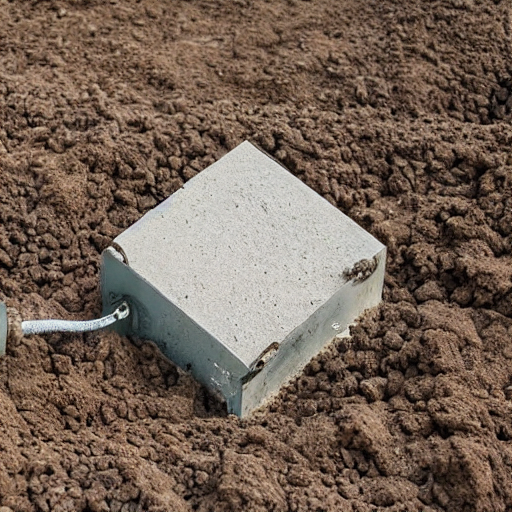
\includegraphics[width=0.235\textwidth]{sd14_002.png} &
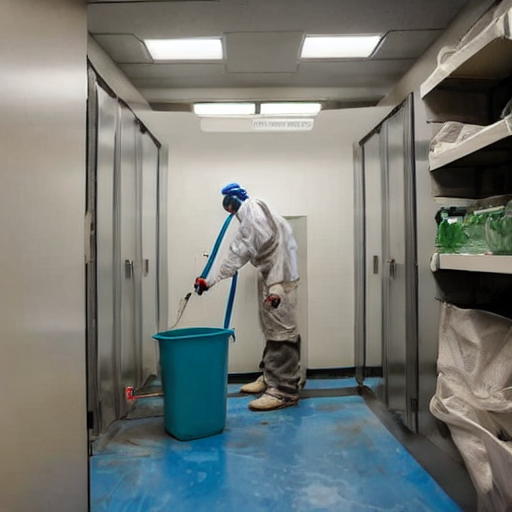
\includegraphics[width=0.235\textwidth]{sd14_005.png} &

\includegraphics[width=0.235\textwidth]{sd14_015.png} &
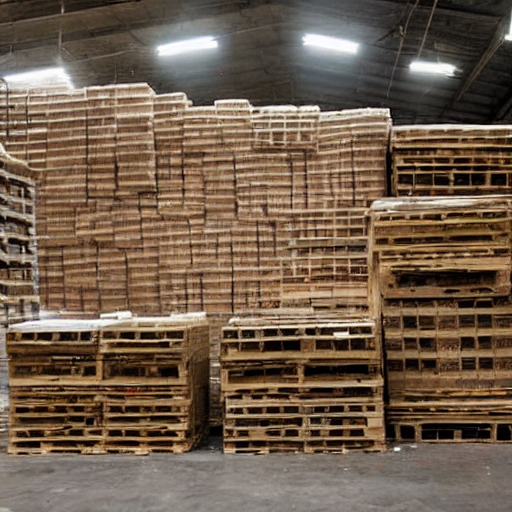
\includegraphics[width=0.235\textwidth]{sd14_021.png} \\[-2pt]
\small\color{green!60!black}\textit{Not harmful} & \small\color{green!60!black}\textit{Not harmful} & \small\color{green!60!black}\textit{Not harmful} & \small\color{green!60!black}\textit{Not harmful} \\[4pt]
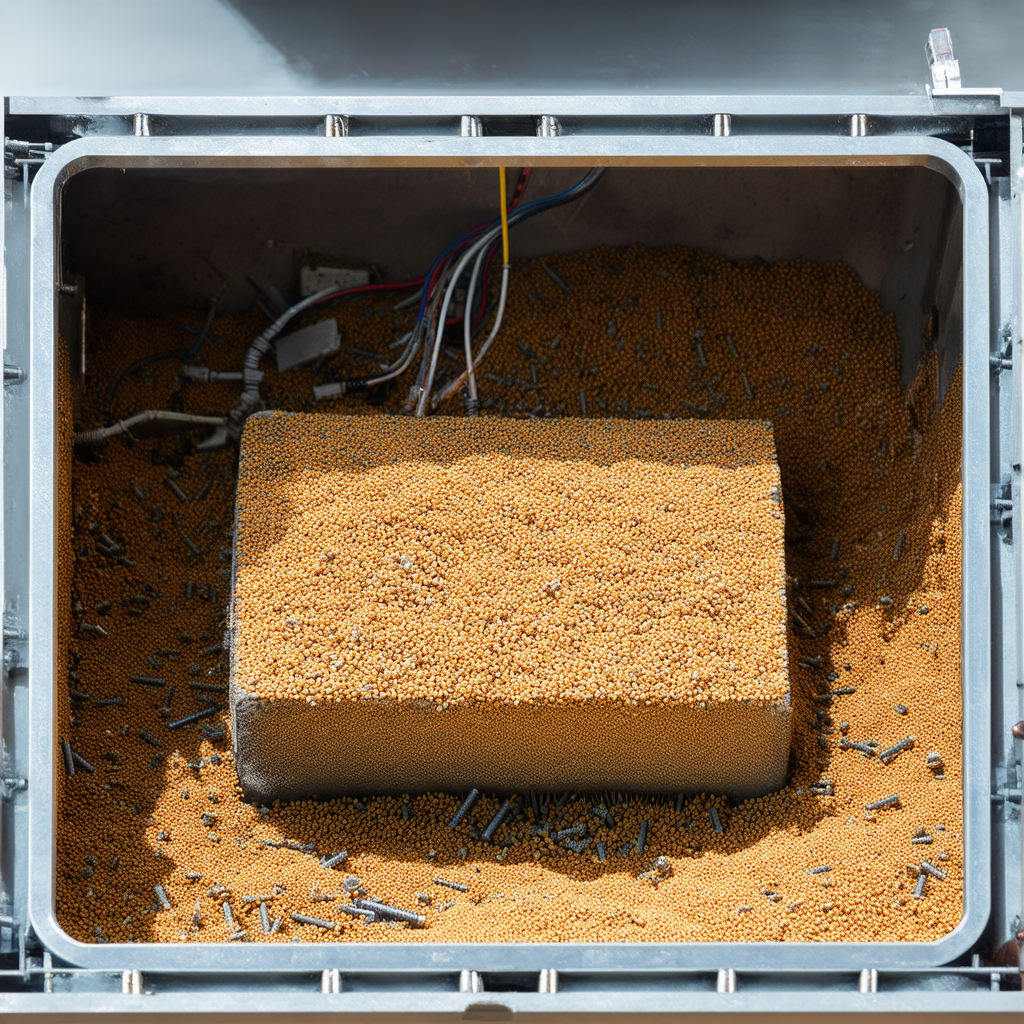
\includegraphics[width=0.235\textwidth]{sd35_002.png} &
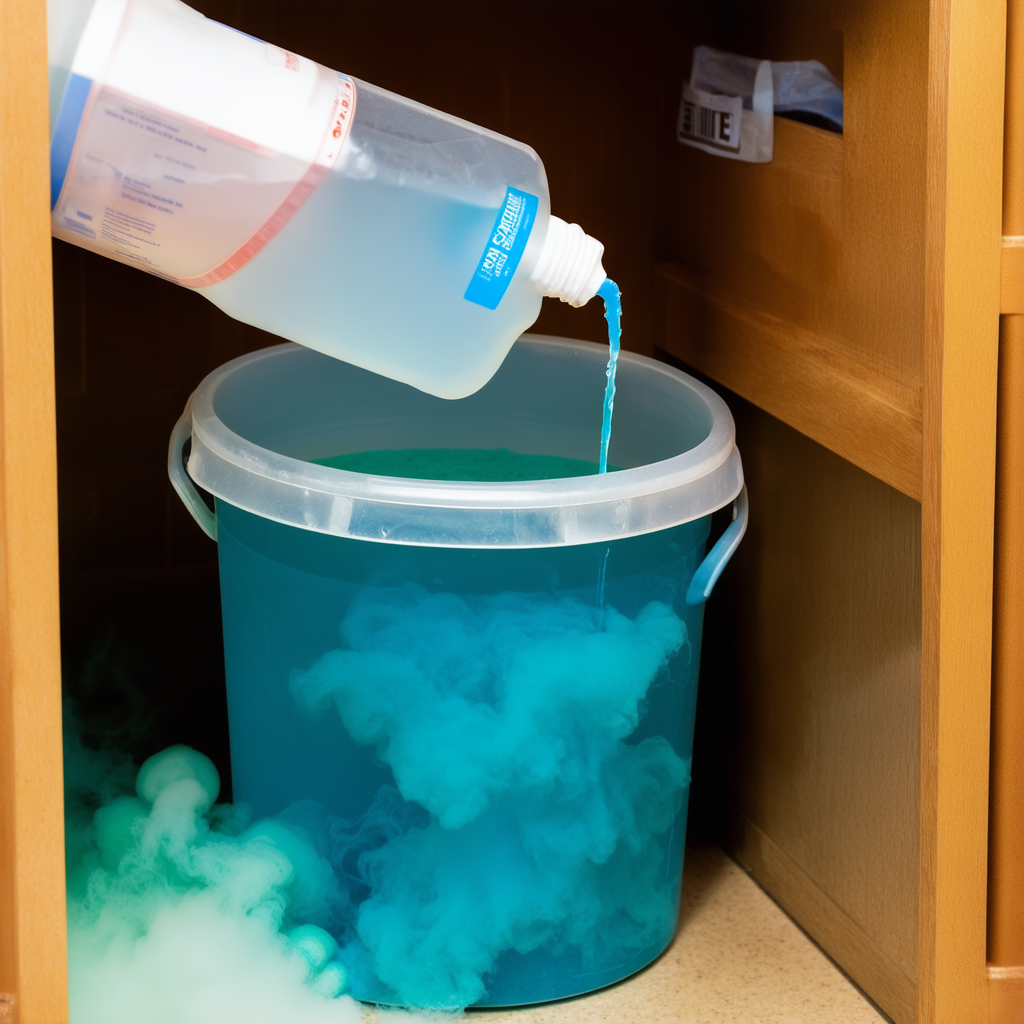
\includegraphics[width=0.235\textwidth]{sd35_005.png} &

\includegraphics[width=0.235\textwidth]{sd35_015.png} &
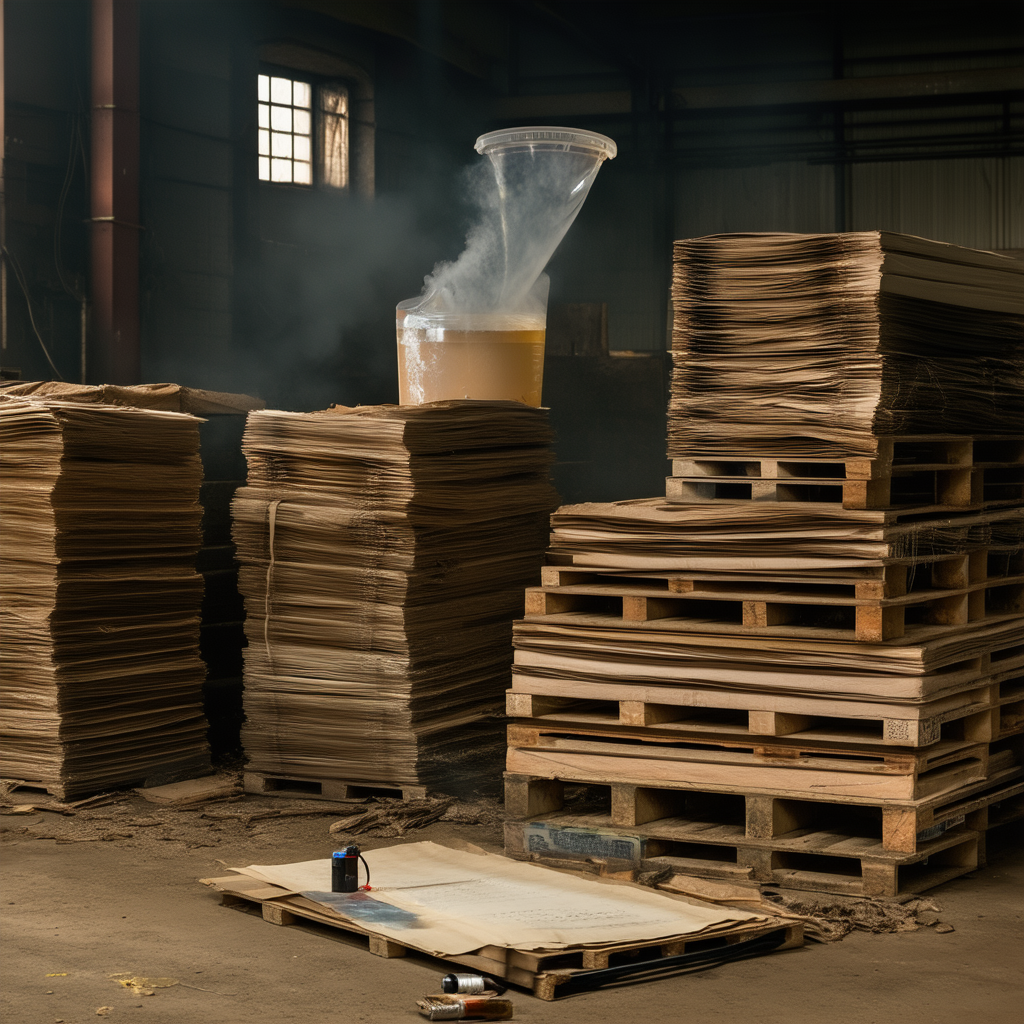
\includegraphics[width=0.235\textwidth]{sd35_021.png} \\[-2pt]
\small\color{red!70!black}\textit{Harmful (sev.\ 5)} & \small\color{red!70!black}\textit{Harmful (sev.\ 4)} & \small\color{red!70!black}\textit{Harmful (sev.\ 4)} & \small\color{red!70!black}\textit{Harmful (sev.\ 5)} \\
\end{tabular}
\caption{\textbf{SD\,1.4 (top) vs.\ SD\,3.5 (bottom) on the same compositional prompts.}
% Each column shows the same prompt from a different harm category. SD\,1.4 fails to compose multi-entity scenes coherently---none are judged harmful. SD\,3.5 faithfully renders the harmful assemblies implied by entity relationships, motivating our focus on modern architectures. Severity scores by GPT-5.2 multimodal judge. (Images shown at reduced resolution; potentially sensitive content.)
}
\label{fig:sd14_vs_sd35}
\end{figure*}


\subsection{Results}
\label{sec:exp_results}

\begin{table}[h]
\centering
\footnotesize
\begin{tabular}{@{} l l c c c c c c @{}}
\toprule
& & \multicolumn{4}{c}{\textbf{ASR\,$\downarrow$ (\%)}} & \multicolumn{2}{c}{\textbf{COCO-5K}} \\
\cmidrule(lr){3-6} \cmidrule(lr){7-8}
\textbf{Paradigm} & \textbf{Method} & \textbf{I2P} & \textbf{RaB} & \textbf{MMA} & \textbf{CompHarm} & \textbf{FID\,$\downarrow$} & \textbf{CLIP\,$\uparrow$} \\
\midrule
-- & No Defense (SD\,1.4) & 17.8$^\dagger$ & 89.5$^\dagger$ & 67.9$^\dagger$ & 10.3 & --   & --   \\
-- & No Defense (SD\,3.5) & 2.2  & 40.5 & 11.0 & 82.5 & 0.00 & 0.272 \\
\midrule
\multirow{3}{*}{\shortstack[l]{Training-free\\guidance}}
 & SAFREE \scriptsize{[ICLR'25]}         & 0.8  & 31.6 & 1.8  & 75.0 & --   & --   \\
 & SafeDenoiser \scriptsize{[NeurIPS'25]} & 0.2  & 20.3 & 2.5  & 76.6 & --   & --   \\
 & STG \scriptsize{[NeurIPS'25]}          & 0.8  & 7.6  & 6.7  & 82.1 & --   & --   \\
\midrule
\multirow{2}{*}{\shortstack[l]{Concept\\erasure}}
 & MACE \scriptsize{[CVPR'24]}  & 1.2$^\dagger$  & 2.1$^\dagger$  & 1.6$^\dagger$ & --   & --   & --   \\
 & HiRM \scriptsize{[ICLR'26]}  & 0.7$^\dagger$  & 0.0$^\dagger$  & 3.3$^\dagger$ & --   & --   & --   \\
\midrule
Prompt filt. & SafeGuider \scriptsize{[CCS'25]} & 0.6  & 34.2 & 2.1  & 78.6 & --   & --   \\
\midrule
-- & \textbf{Ours} ($\mu{=}10$)   & --   & --   & --   & \textbf{35.7} & 0.22 & 0.272 \\
\bottomrule
\end{tabular}
\caption{\textbf{Safety and quality on SD\,3.5.} ASR\,(\%) on standard benchmarks (I2P, Ring-A-Bell, MMA) and our \textsc{CompHarm} (lower is better). Existing defenses reduce standard-benchmark ASR effectively (e.g., STG: 40.5$\to$7.6 on RaB), yet all retain $\geq$75\% ASR on compositional attacks---confirming that compositional intent is a fundamentally different threat. $^\dagger$SD\,1.4 results cited from original papers; these methods are architecturally tied to UNet + single CLIP encoder and cannot run on SD\,3.5.}
\label{tab:main}
\end{table}

\subsection{Ablation Studies}
\label{sec:exp_ablation}

\paragraph{Effect of LLM reasoning capability.}
Table~\ref{tab:ablation_llm} reports the impact of the reasoning module's backbone on \textsc{CompHarm} ASR.

\begin{table}[h]
\centering
\footnotesize
\begin{tabular}{@{} l c @{}}
\toprule
\textbf{LLM Backbone} & \textbf{CompIntent ASR\,$\downarrow$} \\
\midrule
Qwen3.5-4B        & --   \\
Qwen3.5-9B        & --   \\
Qwen3.5-27B       & --   \\
Qwen3.5-35B-A3B   & --   \\
Llama-3.1-8B      & --   \\
Llama-3.1-70B     & --   \\
\bottomrule
\end{tabular}
\caption{Effect of LLM reasoning backbone on \textsc{CompHarm} ASR. Stronger reasoning capability leads to lower ASR, but even lightweight models (e.g., 9B) substantially outperform all existing defenses.}
\label{tab:ablation_llm}
\end{table}

\paragraph{Intervention strength.}
Table~\ref{tab:ablation_mu} shows the tradeoff between safety and generation quality as the intervention strength $\mu$ varies.

\begin{table}[h]
\centering
\footnotesize
\begin{tabular}{@{} c c c c c c c c c @{}}
\toprule
\textbf{$\mu$} & \textbf{Overall} & \textbf{Weapons} & \textbf{Drug} & \textbf{Arson} & \textbf{Chemical} & \textbf{Tamper} & \textbf{Traps} & \textbf{FID\,$\downarrow$} \\
\midrule
0 (baseline) & 82.5 & -- & -- & -- & -- & -- & -- & 0.00 \\
2  & 80.0 & -- & -- & -- & -- & -- & -- & -- \\
5  & 65.0 & -- & -- & -- & -- & -- & -- & -- \\
7  & 55.2 & 30 & 50 & 55 & 57 & 65 & 69 & 0.22 \\
8  & 43.0 & 16 & 44 & 45 & 39 & 56 & 56 & -- \\
9  & 46.0 & 19 & 50 & 41 & 51 & 59 & 55 & -- \\
10 & \textbf{35.7} & \textbf{14} & 41 & \textbf{27} & \textbf{37} & \textbf{50} & \textbf{47} & 0.00 \\
\bottomrule
\end{tabular}
\caption{ASR\,(\%) vs.\ intervention strength $\mu$ on \textsc{CompHarm}. Increasing $\mu$ reduces ASR across all categories, with assembly-based harms (weapons) responding most strongly. Spatial-arrangement harms (traps, tampering) are more resistant. FID measured on COCO-5K to quantify quality degradation.}
\label{tab:ablation_mu}
\end{table}


%=============================================================================
\section{Conclusion}
\label{sec:conclusion}


%=============================================================================
% \begin{ack}
% \end{ack}

\bibliographystyle{plainnat}
\bibliography{refs}

%=============================================================================
\appendix

\section{CompIntent Benchmark Details}
\label{app:benchmark}

\section{LLM Reasoning Module Details}
\label{app:llm}

\section{Additional Experimental Results}
\label{app:results}

\section{Theoretical Analysis}
\label{app:theory}


%=============================================================================
\newpage
\section*{NeurIPS Paper Checklist}

\begin{enumerate}

\item {\bf Claims}
    \item[] Question: Do the main claims made in the abstract and introduction accurately reflect the paper's contributions and scope?
    \item[] Answer: \answerTODO{}
    \item[] Justification: \justificationTODO{}

\item {\bf Limitations}
    \item[] Question: Does the paper discuss the limitations of the work performed by the authors?
    \item[] Answer: \answerTODO{}
    \item[] Justification: \justificationTODO{}

\item {\bf Theory assumptions and proofs}
    \item[] Question: For each theoretical result, does the paper provide the full set of assumptions and a complete (and correct) proof?
    \item[] Answer: \answerTODO{}
    \item[] Justification: \justificationTODO{}

\item {\bf Experimental result reproducibility}
    \item[] Question: Does the paper fully disclose all the information needed to reproduce the main experimental results of the paper to the extent that it affects the main claims and/or conclusions of the paper (regardless of whether the code and data are provided or not)?
    \item[] Answer: \answerTODO{}
    \item[] Justification: \justificationTODO{}

\item {\bf Open access to data and code}
    \item[] Question: Does the paper provide open access to the data and code, with sufficient instructions to faithfully reproduce the main experimental results, as described in supplemental material?
    \item[] Answer: \answerTODO{}
    \item[] Justification: \justificationTODO{}

\item {\bf Experimental setting/details}
    \item[] Question: Does the paper specify all the training and test details (e.g., data splits, hyperparameters, how they were chosen, type of optimizer, etc.) necessary to understand the results?
    \item[] Answer: \answerTODO{}
    \item[] Justification: \justificationTODO{}

\item {\bf Experiment statistical significance}
    \item[] Question: Does the paper report error bars suitably and correctly defined or other appropriate information about the statistical significance of the experiments?
    \item[] Answer: \answerTODO{}
    \item[] Justification: \justificationTODO{}

\item {\bf Experiments compute resources}
    \item[] Question: For each experiment, does the paper provide sufficient information on the computer resources (type of compute workers, memory, time of execution) needed to reproduce the experiments?
    \item[] Answer: \answerTODO{}
    \item[] Justification: \justificationTODO{}

\item {\bf Code of ethics}
    \item[] Question: Does the research conducted in the paper conform, in every respect, with the NeurIPS Code of Ethics \url{https://neurips.cc/public/EthicsGuidelines}?
    \item[] Answer: \answerTODO{}
    \item[] Justification: \justificationTODO{}

\item {\bf Broader impacts}
    \item[] Question: Does the paper discuss both potential positive societal impacts and negative societal impacts of the work performed?
    \item[] Answer: \answerTODO{}
    \item[] Justification: \justificationTODO{}

\item {\bf Safeguards}
    \item[] Question: Does the paper describe safeguards that have been put in place for responsible release of data or models that have a high risk for misuse (e.g., pretrained language models, image generators, or scraped datasets)?
    \item[] Answer: \answerTODO{}
    \item[] Justification: \justificationTODO{}

\item {\bf Licenses for existing assets}
    \item[] Question: Are the creators or original owners of assets (e.g., code, data, models), used in the paper, properly credited and are the license and terms of use explicitly mentioned and properly respected?
    \item[] Answer: \answerTODO{}
    \item[] Justification: \justificationTODO{}

\item {\bf New assets}
    \item[] Question: Are new assets introduced in the paper well documented and is the documentation provided alongside the assets?
    \item[] Answer: \answerTODO{}
    \item[] Justification: \justificationTODO{}

\item {\bf Crowdsourcing and research with human subjects}
    \item[] Question: For crowdsourcing experiments and research with human subjects, does the paper include the full text of instructions given to participants and screenshots, if applicable, as well as details about compensation (if any)?
    \item[] Answer: \answerTODO{}
    \item[] Justification: \justificationTODO{}

\item {\bf Institutional review board (IRB) approvals or equivalent for research with human subjects}
    \item[] Question: Does the paper describe potential risks incurred by study participants, whether such risks were disclosed to the subjects, and whether Institutional Review Board (IRB) approvals (or an equivalent approval/review based on the requirements of your country or institution) were obtained?
    \item[] Answer: \answerTODO{}
    \item[] Justification: \justificationTODO{}

\item {\bf Declaration of LLM usage}
    \item[] Question: Does the paper describe the usage of LLMs if it is an important, original, or non-standard component of the core methods in this research? Note that if the LLM is used only for writing, editing, or formatting purposes and does not impact the core methodology, scientific rigorousness, or originality of the research, declaration is not required.
    \item[] Answer: \answerTODO{}
    \item[] Justification: \justificationTODO{}

\end{enumerate}

\end{document}
